\chapter{Probabilistic Graphical Models}
\label{cha:probabilistic_graphical_models}

In mathematical graph theory a \emph{graph}
\begin{align}
    G &= (\mathcal{V},\mathcal{E}) \\
    \mathcal{V} &= \{V_1,\hdots ,V_n\}
\end{align}
is defined as an ordered pair of a set $\mathcal{V}$ of \emph{vertices} (also \emph{nodes}) and a
set $\mathcal{E}$ of \emph{edges} (also \emph{arcs} if directed) between pairs of vertices
~\citep[34]{koller_09_probabilistic}. Arcs are directed ($V_i\to V_j$), with an arrow pointing from
parent to child node, representing the direction of the interaction, while edges are undirected
($V_i \textbf{ --- } V_j$). More concisely, this implies structure, which can be exploited for
modeling probability distributions as \emph{probabilistic graphical models}. Here, nodes represent
\emph{random variables} and edges describe their independence/dependence
relationships~\citep[57]{barber_12_bayesian}.

The graphical models as defined in \cref{sec:gm-graphical-models} can be utilized to model
tracking-by-assignment problems as described in \cref{cha:gm-in-tracking,cha:joint}. However, as a
first step, \cref{sec:probability-theory} clarifies basic probabilistic concepts that are used
throughout this thesis and defines an unambiguous notation thereof.
% Closely related to
% this are \emph{factor graphs} that can describe factorized probability distributions and are
% especially useful when it comes to inference, \ie extraction of information from the graphical
% model. 

\section{Probability Theory}
\label{sec:probability-theory}
In general, probability reflects the level of confidence that an event will happen. If, for example,
the weather forecast says, that it will rain with a probability of $0.9$ (or $90\%$), it is
advisable to bring weather-proof clothes when going outside. In order to migrate from this
day-to-day life view on probability to a more formal representation, it is necessary to define what
an event is that a probability is assigned to.

First we define a \emph{sample space} $\Omega$ of possible outcomes of a random experiment or
observation~\citep[17]{billingsley_95_probability}. Furthermore,
the non-empty set $\mathcal{S}$ of \emph{measurable events} or \emph{$\sigma$-algebra} contains those outcomes $\mathcal{S} \ni
\alpha \subseteq \Omega$ which we intend to assign probabilities to.
\begin{mydef}[{\citealp[1]{durrett_10_probability}}]
    \label{def:sigma-algebra}
    A \emph{$\sigma$-algebra} $\mathcal{S}$ is a non-empty collection of subsets $\alpha$ of
    $\Omega$ that satisfy
    \begin{enumerate}
          \item $\emptyset \in \mathcal{S} \wedge \Omega \in \mathcal{S}$. \label{itm:sample-space-one}
          \item Closure under union: $\alpha, \beta \in \mathcal{S} \Rightarrow \alpha \cup \beta \in
        \mathcal{S}$ \label{itm:sample-space-two}
          \item Closure under complementation: $\alpha \in \mathcal{S} \Rightarrow \Omega \setminus
        \alpha \in \mathcal{S}$ \label{itm:sample-space-three}
    \end{enumerate}
\end{mydef}
% These constrictions lay the foundations for the definition of a probability distribution.
The pair $(\Omega, \mathcal{S})$ is called a \emph{measurable space}. Then, a \emph{probability
    distribution} can be defined on a measurable space.

\begin{mydef}[{\citealp[17]{koller_09_probabilistic}}]
    \label{def:probability}
    A \emph{probability distribution} $P$ over $(\Omega, \mathcal{S})$
    \begin{align}
        \label{eq:probability-mapping}
        P: \mathcal{S} &\to [0,1] \subset \mathbb{R} \\ \nonumber
        \alpha &\mapsto P(\alpha)
    \end{align}
    maps the outcome $\alpha \in \mathcal{S}$ of a random experiment to a real number $P(\alpha)$ in
    the interval $[0,1]$. In addition, it fulfills the \emph{Kolmogorov axioms}:
    \begin{enumerate}
          \item $P(\alpha) \ge 0 \; \forall \alpha \in \mathcal{S}$
          \item $P(\Omega) = 1$ \label{itm:probability-trivial}
          \item $\alpha, \beta \in \mathcal{S} \wedge \alpha \cap \beta = \emptyset \Rightarrow
        P(\alpha \cup \beta) = P(\alpha) + P(\beta)$ \label{itm:probability-union}
    \end{enumerate}
\end{mydef}
Note that the second and third of the Kolmogorov axioms impose normalization of the probability
distribution and assign zero probability to the empty event:
\begin{align}
    \label{eq:probability-no-empty-event}
    &&P(\Omega) = P(\Omega \cup \emptyset) = P(\Omega) + P(\emptyset) \\
    &\Leftrightarrow &P(\Omega) - P(\Omega) = P(\Omega) - P(\Omega) + P(\emptyset) \\
    &\Leftrightarrow &P(\emptyset) = 0
\end{align}
The Bayesian interpretation sees probability as a degree of confidence in between the two extrema
$P(\alpha)=1$ and $P(\alpha)=0$ for event $\alpha \in \mathcal{S}$ as an outcome of a random
experiment. From a frequentist point of view, that is the fraction of outcomes in the limit of
infinite repetitions of the random experiment.

% When the quantity of interest is not the probability of an event $\beta$, but the probability
% of event $\beta$ given the knowledge about event $\alpha$, or -- more formal -- conditioned on event
% $\alpha$, 
\begin{mydef}[{\citealp[18]{koller_09_probabilistic}}]
    \label{def:conditional-probability}
    \emph{The conditional} probability of $\beta$ given $\alpha$
    \begin{align}
        \label{eq:condititonal-probability}
        P(\beta | \alpha) = \frac{P(\alpha \cap \beta)}{P(\alpha)}, \; P(\alpha) \ne 0
    \end{align}
    is the probability that $\beta$ will happen, given knowledge about
    $\alpha$.
\end{mydef}
Notably, $P(\beta | \alpha)$ fulfills all requirements from \cref{def:probability} and therefore is
a probability distribution.

A direct consequence of \cref{eq:condititonal-probability} is \emph{Bayes' theorem}~\citep[15]{bishop_07_pattern}:
\begin{align}
    \label{eq:bayes-theorem}
    P(\alpha|\beta)P(\beta) = P(\beta|\alpha)P(\alpha)
\end{align}
    

% \label{sec:probability-theory}
% \begin{mydef}
%     \label{def:gm-space}
%     The \emph{sample space} $\Omega$ consists of all possible outcomes $\omega$ of a random experiment or
%     observation\citep{billingsley_95_probability}~\citep[17]{billingsley_95_probability}. 
% \end{mydef}

% \citet{billingsley_95_probability}{17}

Hitherto, \cref{def:probability} provides a distribution over the abstract space of events $\alpha
\in \mathcal{S}$ that are sets of possible outcomes ($\alpha \subseteq \Omega$). For the application
on real world problems, it is more intuitive to model distributions over attributes of the outcome
rather than the outcome itself. Then, \emph{random variables} provide the means to inject attributes
of the outcome.

\begin{mydef}[{\citealp[8]{durrett_10_probability}}]
    \label{def:random-var}
    A \emph{random variable} $X$ is a function
    \begin{align}
        \label{eq:random-var}
        X:\Omega &\to \val(X) \\
        \omega &\mapsto X(\omega) = x
    \end{align}
    that assigns a realization $x$ of the random variable $X$ to the outcome of a random
    experiment. Here, $\val(X)$ denotes the range of values that
    $X$ can take, most commonly real or natural numbers or subsets thereof.
\end{mydef}
Throughout this thesis, random variables are denoted by a capital letter with realizations depicted
by the appropriate lower case counterpart.
% Furthermore, all random variables take discrete values,
% \ie $\val(X) \subset \mathbb{N} \cup \{0\}$ and $|val(X)| = m < \infty$, unless stated
% otherwise.
Then, 
\begin{align}
    P(X=x)=P\left(\{\omega \in \Omega : X(\omega) = x\}\right)
\end{align}
is the probability that random variable $X$ takes the value $x$ and
\begin{align}
    \sum_{X} = \sum_{x \in \val(X)}
\end{align}
denotes summation over all possible values of $X$. With the introduced convention that a random
variable and its realization form a pair of corresponding lower case and upper case letters, it is
obvious that $x$ always refers to the realization of random variable $X$. Thus, $P(X=x)$ can be
written as $P(x)$ for brevity, when appropriate. Furthermore, sets of random variables are denoted
by calligraphic letters. In general, it is sensible to form sets of random variables that have the
same range of values or that can be grouped semantically. As a final abbreviation, $P(X=x,Y=y)$ and
$P(x,y)$ are shortcuts for the \emph{joint distribution} over $X$ and $Y$ $P\left((X=x) \cap
    (Y=y)\right)$. More generally, this holds for a joint distribution of any number of random
variables: $P(x_1,\hdots,x_N) = P\left(\bigcap_{i=1}^N(X_i=x_i)\right)$. These notational details
are subsumed in \cref{tab:probability-notation}.

In the following, properties of probability distribution over discrete random variables are
introduced. In a similar fashion and with slight modifications, these properties hold for continuous
random variables as well: Sums are exchanged for integrals and the properties are described in terms
of a \emph{probability density function}, typically denoted by $p(\cdot)$, instead of the
probability distribution. In this context, it is important to note that, formally, a distribution
over a continuous random variable describes the probability that the random variable takes a value
in a specified interval rather than a certain value. In spite of this distinction, the probability
density function is commonly referred to as probability distribution. For discrete variables,
however, the intuitive interpretation of assigning probabilities to the states of a random variable
holds. A more in depth presentation of distributions in general and distributions over continuous
random variables in particular can be found in
\citet{durrett_10_probability,billingsley_95_probability,chung_68_course}.

\begin{table}
    \centering
    \begin{tabular}{ll}
        \toprule
        Notation & Meaning \\ \midrule
        $X$ & random variable \\
        $\val(X)$ & value range of $X$ \\
        $X \in A$ & short for $\val(X)=A$ \\
        $x$ & realization of $X$ \\
        $P\left(\{\omega \in \Omega : X(\omega) = x\}\right)$  & probability of $X$ to take value $x$ \\
        $P(X=x)$ & $P\left(\{\omega \in \Omega : X(\omega) = x\}\right)$ \\
        $P(x)$ & $P(X=x)$ \\
        $\mathcal{X}$ & set of random variables $\{X_i\}_{i=1,\hdots,N}$ \\
        $P\left(\bigcap_{i=1}^N(X_i=x_i)\right)$ & joint distribution over set of
        $N$ random variables \\ 
        $P(x_1,\hdots,x_N)$ & $ P\left(\bigcap_{i=1}^N(X_i=x_i)\right)$ \\
        $\sum_{\mathcal{X}}$ & Summation over all possible states of $\mathcal{X}$ \\
        \bottomrule
    \end{tabular}
    \caption[Probability: Notations]{Notations and abbreviations for random variables and probability distributions.}
    \label{tab:probability-notation}
\end{table}

\begin{mydef}
    \label{def:marginalization}
    Given a set of random variables $\mathcal{X} = \{X_1,\hdots,X_N\}$, a \emph{marginal
        distribution} is a probability distribution on a subset of variables
    $\{\hat{X}_1,\hdots,\hat{X}_M\} = \hat{\mathcal{X}} \subset \mathcal{X}$, such that
    \begin{align}
        \label{eq:marginalization}
        P(\hat{x}_1,\hdots,\hat{x}_M) &= \sum_{X_{i_1}}\cdots\sum_{X_{i_{N-M}}}P(x_1,\hdots,x_N), \\
        \left\{X_{i_k}\right\}_{k=1,\hdots,N-M} &= \mathcal{X} \setminus \mathcal{\hat{X}}.
    \end{align}
\end{mydef}
Here, the set $\left\{X_{i_k}\right\}_{k=1,\hdots,N-M}$ denotes all random variables that are in the
original set of variables $\mathcal{X}$, but not in its subset $\hat{\mathcal{X}}$. These $N-M$
variables are ``marginalized out'' by summation over their $N-M$ value ranges. For the purpose of
explanation, take the distribution $P(x, y)$ over two random variables $X$ and $Y$ as an
example. Marginalizing over $Y$ then results in the distribution
\begin{align}
    \label{eq:probability-marginal-example}
    P(x) = \sum_{y \in \val(Y)}P(x, Y=y).
\end{align}
This example is visualized in \cref{fig:probability-example-marginal} with $\val(X)=\{x \in
\mathbb{N} : x \le 9\}$ and \mbox{$\val(Y)=\{1, 2\}$}. In addition,
\cref{fig:probability-example-conditional} shows a conditional distribution of $P(x,y)$. Note that
for random variables conditional probability
\begin{align}
    \label{eq:random-variable-conditional}
    P(x|y) = \frac{P(x,y)}{P(y)}
\end{align}
is defined analogously to \cref{def:conditional-probability}. Therefore, Bayes' theorem
(\cref{eq:bayes-theorem})
\begin{align}
    \label{eq:bayes-theorem-rv}
    P(x|y)P(y) = P(y|x)P(x)
\end{align}
holds for random variables as well. The different natures of a marginal distribution and a
conditional distribution is visualized in \cref{fig:probability-vis}. Once again, this visualization
stresses that, generally speaking, marginalizing and conditioning are not the same. However, when
equality holds, $X$ and $Y$ are considered marginally independent (\cref{eq:probability-marginal-independence-v2}).
\begin{mydef}[{\citealp[10]{barber_12_bayesian}}]
    \label{def:independence}
    Two variables $X$ and $Y$ are \emph{marginally independent} if their joint probability
    factorizes into the product of their marginals:
    \begin{align}
        \label{eq:probability-marginal-independence}
        P(x,y) = P(x)P(y).
    \end{align}
    Then, $X \independent Y$ denotes marginal independence of $X$ and $Y$. The generalization to
    sets of variables $\mathcal{X}$ and $\mathcal{Y}$ can be formulated likewise:
    \begin{align}
        \label{eq:probability-marginal-independence-sets}
        P(x_1,\hdots x_N, y_1,\hdots, y_M) = P(x_1,\hdots x_N)P(y_1,\hdots, y_M)
    \end{align}
\end{mydef}
The abstract \cref{def:independence} can be interpreted meaningfully in that sense, that knowledge
of $Y$ does not change the probability for $X$. Moreover, combining
\cref{eq:bayes-theorem-rv,eq:probability-marginal-independence} for non-zero distributions $P(x) \ne
0$ and $P(y) \ne 0$, yields
\begin{align}
    \label{eq:probability-marginal-independence-v2}
    P(x|y) = P(x) \;\forall y \Leftrightarrow P(y|x) = P(y) \; \forall x,
\end{align}
a mathematical formulation of this interpretation. In \cref{fig:probability-example-joint}, the
distribution over $X$ is clearly dependent on the choice of $Y$: The distribution over $X$ in the
bottom row differs from the distribution over $X$ in the top row. Thus, $X$ and $Y$ are not marginally
independent, $X \not \independent Y$.

More often than being marginally independent, sets of variables are independent conditioned on an
additional set of variables.
\begin{mydef}[{\citealp[7]{barber_12_bayesian}}]
    \label{def:probability-conditional-independence}
    Let $\mathcal{X}$, $\mathcal{Y}$, $\mathcal{Z}$ be sets of random variables. Then $\mathcal{X}$
    and $\mathcal{Y}$ are called \emph{conditionally independent} on $\mathcal{Z}$ under the
    distribution P, if P satisfies
    \begin{align}
        \label{eq:conditional-independence}
        P(\mathcal{X}, \mathcal{Y}|\mathcal{Z}) =
        P(\mathcal{X}|\mathcal{Z})P(\mathcal{Y}|\mathcal{Z}).
    \end{align}
    Conditional independence $\mathcal{X} \independent \mathcal{Y} \;|\; \mathcal{Z}$ is denoted in the
    same manner as marginal dependence.
\end{mydef}
Note that the formulation \cref{eq:conditional-independence} allows for formulating marginal
independency in terms of conditional independency: Two sets of variables $\mathcal{X}$ and
$\mathcal{Y}$ are marginally independent if they are independent conditioned on the empty set, or
formally
\begin{align}
    \label{probability-conditional-marginal}
    \mathcal{X} \independent \mathcal{Y} \; | \; \emptyset \Leftrightarrow \mathcal{X} \independent \mathcal{Y}.
\end{align}

Finally, the normalization requirement from \cref{def:probability} holds for probability
distributions over random variables by demanding
\begin{align}
    \label{eq:probability-normalization}
    \sum_{x \in \val(X)}P(x) = 1.
\end{align}



\begin{figure}
    \centering
    % \begin{subfigure}[t]{0.08\textwidth}
    %     \nonumber
    %         \vspace{0pt}
    %         \raggedright
    %         $Y=2$ \\
    %         $Y=1$
    %     \end{subfigure}
    \begin{subfigure}[b]{0.3\textwidth}
        \centering
        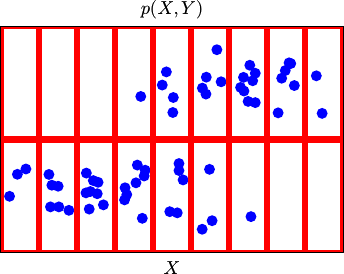
\includegraphics[width=\textwidth]{images/probability/joint.png}
        \caption{$P(X=x,Y=y)$}
        \label{fig:probability-example-joint}
    \end{subfigure}
    ~
    \begin{subfigure}[b]{0.3\textwidth}
        \centering
        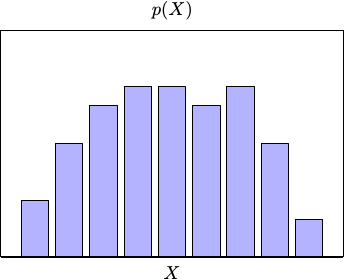
\includegraphics[width=\textwidth]{images/probability/marginal-x.png}
        \caption{$P(X=x)$}
        \label{fig:probability-example-marginal}
    \end{subfigure}
    ~
    \begin{subfigure}[b]{0.3\textwidth}
        \centering
        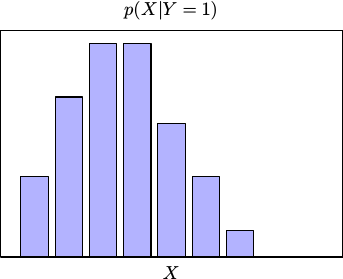
\includegraphics[width=\textwidth]{images/probability/conditional-on-y.png}
        \caption{$P(X=x|Y=1)$}
        \label{fig:probability-example-conditional}
    \end{subfigure}
    \caption[Example for joint distribution with marginal and conditional
    distribution]{Visualization of marginal (\subref{fig:probability-example-marginal}) and
        conditional (\subref{fig:probability-example-conditional}) distributions of a joint
        probability distribution (\subref{fig:probability-example-joint}) over two variables $X$ and
        $Y$ (taken and modified from \citealp[16]{bishop_07_pattern}). $X$ takes nine
        possible values, $Y$ takes two possible values ($1$ and $2$, from bottom to top). Clearly
        (\subref{fig:probability-example-marginal}) and
        (\subref{fig:probability-example-conditional}) are two different distributions and
        therefore visualize the difference between marginal and conditional distribution:
        Marginalizing over $Y$ corresponds to adding the value of each point in
        (\subref{fig:probability-example-joint}) to the corresponding bin in the histogram over $X$
        in (\subref{fig:probability-example-marginal}). The resulting distribution is not a function
        of $y$. On the contrary, conditioning $Y=1$ can be understood as selecting only that part of
        the distribution that fulfills that condition, \ie the bottom row in
        (\subref{fig:probability-example-joint}). In order to arrive at the conditional distribution
        (\subref{fig:probability-example-conditional}), the selected row needs to be normalized by
        the probability $P(Y=1)$.}
    \label{fig:probability-vis}
\end{figure}

Queries on a probability distribution for drawing conclusions are called
\emph{inference}~\citep[75]{barber_12_bayesian}. A simple query is the calculation of the
probability for a specific state of random variables. In the context of data observation, the
posterior
\begin{align}
    \label{eq:probability-posterior}
    P(\mathcal{X}|\mathcal{D}) = \frac{P(\mathcal{D}|\mathcal{X})}{P(\mathcal{D})}
\end{align}
is the distribution of random variables $\mathcal{X}$ conditioned on observations
$\mathcal{D}$~\citep[173]{barber_12_bayesian}. The mode of the posterior distribution, \ie the
variable setting
\begin{align}
    \mathcal{X}^{\text{MAP}} = \argmax_{\mathcal{X}} P(\mathcal{X}|\mathcal{D}),
\end{align}
which maximizes the posterior distribution, is called the \emph{maximum a posteriori} (MAP)
estimate. Throughout this thesis, the explicit statement of conditioning on observed data
$\mathcal{D}$ is omitted.

With the introduction of and notational conventions~(\cref{tab:probability-notation}) for random
variables and probabilities at hand, we continue with a short introduction to probabilistic
graphical models in \cref{sec:gm-graphical-models}.

% For the models presented in this thesis, the
% \emph{maximum a posteriori} (MAP) estimate~\citep[173]{barber_12_bayesian}
% \begin{align}
%     \label{eq:probability-map}
% \end{align}
% is used to infer the mode of the associated posterior probability distributions.



% A distribution $P(\mathcal{X}=\{x_1,\hdots,x_N\})=P(x_1,\hdots,x_n)$ over a set of random variables
% $\mathcal{X}=\{X_1,\hdots,X_n\}$ is called a \emph{joint distribution}. 

% \cref{def:random-var} allows for the definition of joint distributions over random variables. Due to
% the limitation to discrete random variables, all definitions refer to discrete random variables
% only. However, these definitions can be applied to conitinuous variables with only slight
% modifications (see \citet[Chapter~1]{barber_12_bayesian} and
% \citet[Chapter~2.1]{koller_09_probabilistic}). 


% Throughout this thesis we encounter only probability distributions over discrete random
% variables. Thus, without the need for an explicit declaration, all random variables are constrained
% to be discrete (including binary random variables). Furthermore, only properties of distributions over
% discrete random variables are described in the following. However, this properties hold for
% continuous random variables as well with the slight m



%%% Local Variables: 
%%% mode: latex
%%% TeX-master: "../../main"
%%% End: 

\section{Graphical Models}
\label{sec:gm-graphical-models}

A graphical representation of probability distributions is helpful for modeling
independence/dependence relationships. Graphical models impose structure that reflects those
relations. However, the capabilities of graphical models is limited and any use case requires the
choice of an appropriate kind of graphical model \citep[57]{barber_12_bayesian}. Of
the many types of graphical models we present Bayesian networks (\cref{subsec:gm-bayesian-net}),
conditional random fields (\cref{subsec:gm-crf}) and factor graphs
(\cref{subsec:factor-graphs}). Both the Bayesian networks and the conditional random fields can be
transformed into a factor graph representation, which is commonly used for inference. Moreover, as
shown in \cref{subsec:fg-conservation} and \cref{cha:joint}, a factor graph can also be utilized for
modeling.

\subsection{Bayesian Networks}
\label{subsec:gm-bayesian-net}

Bayesian Networks are graphical models that are used for modeling causal independencies. The
structure of the graph defines the conditional dependencies of the underlying distribution.

\begin{mydef}[{\citealp[37]{barber_12_bayesian}}]
    A \emph{Bayesian network}, also \emph{belief network} or \emph{directed acyclic graphical model}
    (DAG), is a graphical model that describes the distribution
    \begin{align}
        \label{eq:gm-bayesian-net}
        P(\mathcal{X}) = \prod_{X \in \mathcal{X}}P\left(X=x|\pa(X)\right).
    \end{align}
    over a set of random variables $\mathcal{X}$. In the graph representation
    \begin{align}
        G = (\mathcal{V}, \mathcal{A}),
    \end{align}
    each vertex $V \in \mathcal{V}$ represents the distribution over a random variable $X_V \in
    \mathcal{X}$ conditioned on the set of parental variables of $X_V$ as indicated by arrows from
    each parent to child $V$.
    % a random variable $X_V \in \mathcal{X}$. Furthermore,
    % the set of arcs $\mathcal{A}$ is constructed in a way, such that the parents of each node
    % $X_{V_i}\in\mathcal{X}$ are the $M$ vertices $\{V_1,\hdots,V_M\}$ that represent the random
    % variables that $X_{V_i}$ is conditioned on.
\end{mydef}

In that context, $\pa(X_V)$ is the set of parental variables for the random variable
$X_V\in\mathcal{X}$. In terms of a directed acyclic graph
$G=\left(\mathcal{V},\mathcal{A}\right)$, this is the set of all random variables represented by
nodes with an arc pointing to $V$
\begin{align}
    \label{gm-bayesian-parental}
    \pa(X_V) = \left\{X_{V_i} \in \mathcal{X} : (V_i \to V) \in \mathcal{A} \right\}.
\end{align}
This structure is visualized by a toy example in \cref{fig:gm-bayesian-net}.  Furthermore, it can be
exploited to determine conditional independencies of the random variables. In this regard,
\citet{verma_88_causal} introduced the algorithm called \emph{d-separation} for the conclusion of
conditional dependencies from a DAG. \citet[43]{barber_12_bayesian} provides a more compact
description of the method.
\begin{figure}
    \centering
    \begin{subfigure}[t]{0.48\textwidth}
        \centering
        \begin{tikzpicture}[thick, on grid, every node/.style={font=\small, scale=1.5}, baseline=(v.south)]
            \begin{scope}
    \node[RVnode] (v) {$X_1$};
    \node[RVnode, above=of v.north] (v1) {$X_2$};
    \node[RVnode, xshift=-40] at ($(v)!0.5!(v1)$) (h) {$X_3$};
    \path (h) edge[connect] (v);
    \path (h) edge[connect] (v1);
\end{scope}

%%% Local Variables: 
%%% mode: latex
%%% TeX-master: "../../main"
%%% End: 

        \end{tikzpicture}
        %\rule{\textwidth}{0.3pt}
        \caption{Bayesian network: Both $X_1$ and $X_2$ have $X_3$ as a parent.}
        \label{subfig:gm-bayesian-net-example}
    \end{subfigure}
    ~
    \begin{subfigure}[t]{0.48\textwidth}
        \centering
        \begin{tikzpicture}[thick, on grid, every node/.style={font=\small, scale=1.5}, baseline=(v.south)]
            \begin{scope}
    \node[RVnode] (v) {$X_1$};
    \node[RVnode, above=of v.north] (v1) {$X_2$};
    \node[RVnode, xshift=-40] at ($(v)!0.5!(v1)$) (h) {$X_3$};
    \node[Factor, label={[font=\tiny]below left:$\phi_1(x_1,x_3)$}] (f1) at ($(v)!0.5!(h)$) {};
    \node[Factor, label={[font=\tiny]above left:$\phi_2(x_2,x_3)$}] (f2) at ($(v1)!0.5!(h)$) {};
    \node[Factor, label={[font=\tiny]left:$\phi_3(x_1)$}, left=of h.west] (f3) {};
    \factoredge {v, h} {f1} {};
    \factoredge {v1, h} {f2} {};
    \factoredge {h} {f3} {};
\end{scope}

%%% Local Variables: 
%%% mode: latex
%%% TeX-master: "../../main"
%%% End: 

        \end{tikzpicture}
        %\rule{\textwidth}{0.3pt}
        \caption{Factor graph (\cref{subsec:factor-graphs}) representation of
            \cref{subfig:gm-bayesian-net-example}.}
        \label{subfig:gm-bayesian-net-fg}
    \end{subfigure}
    \caption[A simple Bayesian network]{A simple Bayesian network
        (\subref{subfig:gm-bayesian-net-example}) representing the distribution $P(x_1,x_2,x_3) =
        P(x_1|x_3)P(x_2|x_3)P(x_3)$ and a factor graph representation (\subref{subfig:gm-bayesian-net-fg}) $P(x_1, x_2, x_3) =
        \frac{1}{Z}\phi_1(x_1,x_3)\phi_2(x_2,x_3)\phi_3(x_3)$.}
    \label{fig:gm-bayesian-net}
\end{figure}



%%% Local Variables: 
%%% mode: latex
%%% TeX-master: "../../main"
%%% End: 

\subsection{Conditional Random Fields}
\label{subsec:gm-crf}

Conditional random fields (CRFs) are useful for modeling conditional distributions
$P(\mathcal{Y}|\mathcal{X})$ over random output variables $(\mathcal{Y}$) conditioned on the random
input variables $\mathcal{X}$~\citep[142]{koller_09_probabilistic}. In order to
formally define CRFs, we first introduce \emph{cliques}, \emph{Markov networks} and the \emph{Markov
    property}.

\begin{mydef}[{\citealp[23]{barber_12_bayesian}}]
    \label{def:clique}
    In an undirected graph $G = (\mathcal{V}, \mathcal{E})$, a \emph{clique} is a fully connected
    subset of the vertices $\mathcal{V}_c\subseteq\mathcal{V}$, \ie there is a pairwise edge between
    all members of $\mathcal{V}_c$, or more formally: $\exists (V_i \textbf{ --- } V_j) \in
    \mathcal{E}\; \forall \; V_i \ne V_j \in \mathcal{V}_c$. A clique is called \emph{maximal
        clique}, if, for all vertices that are not in the clique $\mathcal{V} \setminus
    \mathcal{V}_c$, the union $\mathcal{V}_c^{\prime} = \mathcal{V}_c \cup \{V_a : V_a \in
    \mathcal{V} \setminus \mathcal{V}_c\}$ of the clique with an arbitrary vertex is not a
    clique. The largest maximal clique in a graph is called the \emph{maximum clique}.
\end{mydef}

With \cref{def:clique}, we now can define a \emph{Markov network} and its graph representation.

\begin{mydef}[{\citealp[59]{barber_12_bayesian}}]
    \label{def:markov-network}
    A \emph{Markov network} over random variables $\mathcal{X}$ is a distribution that factorizes
    into non-negative potentials (functions) $\phi_i(\mathcal{X}_i)$ on subsets of the random
    variables $\mathcal{X}_i\subseteq\mathcal{X}$:
    \begin{align}
        \label{eq:markov-network}
        P(\mathcal{X}) = \frac{1}{Z}\prod_{i=1}^N\phi_i(\mathcal{X}_i)
    \end{align}
    The constant $Z$ ensures normalization. In an undirected graph representation $G$, the subsets
    of variables $\mathcal{X}_i\subseteq\mathcal{X}$ correspond to the maximal cliques in $G$.
\end{mydef}
The Markov property can be defined in terms of a Markov network.
\begin{mydef}[{\citealp[61]{barber_12_bayesian}; \citealp[16]{hammersley_71_markov}}]
    \label{def:markov-property}
    Let ($\mathcal{A}\subseteq\mathcal{X}$, $\mathcal{B}\subseteq\mathcal{X}$,
    $\mathcal{S}\subseteq\mathcal{X}$), represented by vertices ($\mathcal{V}_{\mathcal{A}}$,
    $\mathcal{V}_{\mathcal{B}}$, $\mathcal{V}_{\mathcal{S}}$), be a set of disjoint subsets of
    variables of a Markov network. Then, the \emph{Markov property} states that $\mathcal{A}
    \independent \mathcal{B} | \mathcal{S}$, if there is no path from a member of
    $\mathcal{V}_{\mathcal{A}}$ to a member of $\mathcal{V}_{\mathcal{B}}$ or if every path of any
    member of $\mathcal{V}_{\mathcal{A}}$ to any member of $\mathcal{V}_{\mathcal{B}}$ passes
    through $\mathcal{V}_{\mathcal{S}}$).
\end{mydef}

In particular, % for positive potentials $\phi_k > 0$,
a random variable in a Markov network conditioned on its neighbors is independent of the remaining
variable:
\begin{align}
    \label{eq:local-markov-property}
    P(X|\mathcal{X}\setminus X) = P(X|\neighbor(X)) \\
    \neighbor(X) = \{X^{\prime} \in \mathcal{X} : \exists (V^{\prime} \textbf{ --- } V) \in \mathcal{E}\}
\end{align}
With the knowledge about Markov networks, \emph{conditional random fields} can be defined in terms
of undirected graphical models.

\begin{mydef}[{{\citealp[234]{barber_12_bayesian}; \citealp[3]{lafferty_01_conditional}}}]
    \label{def:crf}
    Let $\mathcal{X}$ be a set of observable (input) random variables and $\mathcal{Y}$ be a set of
    label (output) random variables. Then a \emph{conditional random field} is a conditional
    distribution
    \begin{align}
        \label{eq:crf}
        P(\mathcal{Y}|\mathcal{X}) = \frac{1}{Z(X)}\prod_k\phi(\mathcal{Y}_k, \mathcal{X}_k)
    \end{align}
    over the output $\mathcal{Y}$ conditioned on the input $\mathcal{X}$ that factorizes into
    non-negative potentials $\phi_k$. A CRF can be seen as a Markov network on the output variables
    $\mathcal{Y}$ conditioned on the input $\mathcal{X}$ with a graphical representation
    $G=(\mathcal{V}, \mathcal{E})$. More precisely, the set of vertices
    $\mathcal{V}=\{\mathcal{V}_{\mathcal{Y}}, \mathcal{V}_{\mathcal{X}}\}$ comprises the subsets
    that form vertices representing output variables $\mathcal{V}_{\mathcal{Y}}$ and input variables
    $\mathcal{V}_{\mathcal{X}}$. Therefore, the Markov property holds for $\mathcal{Y}$ conditioned
    on $\mathcal{X}$ with $G_{\mathcal{Y}}=(\mathcal{V}_{\mathcal{Y}}, \mathcal{E}_{\mathcal{Y}})$.
    % Let $G = (\mathcal{V}, \mathcal{E})$ be an undirected graph, whose vertices $V\in\mathcal{V}$
    % index a set of random variables $Y_V \in \mathcal{Y}$ over labels, and a set of random variables
    % $\mathcal{X}$ over observations. Furthermore, the Markov property holds for $\mathcal{Y}$
    % conditioned on $\mathcal{X}$. Then $(X,Y)$ is a \emph{conditional random field}.
    % \begin{align}
    %     \label{eq:gm-crf}
    %     p(\mathcal{Y}|\mathcal{X}) = \frac{1}{Z(\mathcal{X})}\prod_k\phi_k(\mathcal{Y}_k, \mathcal{X}_k)
    % \end{align}
    % over observed variables $\mathcal{X}$ and random variables $\mathcal{Y}$ consisting of $k$
    % factors $phi_k$ that are non-negative functions of subsets $\mathcal{X}_k \subseteq \mathcal{X}$
    % and $\mathcal{Y}_k \subseteq \mathcal{Y}$.
\end{mydef}
Normalization is ensured in \cref{eq:crf} by division by the partition function
\begin{align}
    \label{eq:gm-crf-partition}
    Z(\mathcal{X}) = \sum_{\mathcal{Y}}\prod_k\phi_k(\mathcal{Y}_k, \mathcal{X}_k),
\end{align}
which is calculated by summation over all possible states of the output variables $\mathcal{Y}$.

\begin{figure}
    \centering
    \begin{subfigure}{0.48\textwidth}
        \centering
        \begin{tikzpicture}[thick, on grid, every node/.style={font=\small, scale=1.5}, baseline=(v.south)]
            \begin{scope}
    \node[RVnode] (v) {$y_1$};
    \node[RVnode, above=of v.north] (v1) {$y_2$};
    \node[RVnode, xshift=-40, fill=black!30] at ($(v)!0!(v1)$) (h) {$x_1$};
    \node[RVnode, xshift=-40, fill=black!30] at ($(v)!1!(v1)$) (h1) {$x_2$};
    \path (h) edge (v);
    \path (h1) edge (v1);
    \path (v) edge (v1);

\end{scope}


%%% DIRTY HACK TO ALLOW FOR CAPTIONS AT SAME POSITION!
\begin{scope}[on background layer]
    \node[Factor, color=black!0, label={[font=\tiny, xshift=7, yshift=-7, color=black!0]below:$\psi_1(x_1,y_1)$}] (f1) at
    ($(v)!0.5!(h)$) {};
    \node[Factor, color=black!0, label={[font=\tiny, xshift=7, yshift=7, color=black!0]above:$\psi_1(x_1,y_1)$}] (f2) at
    ($(v1)!0.5!(h1)$) {};
    
\end{scope}

%%% Local Variables: 
%%% mode: latex
%%% TeX-master: "../../main"
%%% End: 

        \end{tikzpicture}
        %\rule{\textwidth}{0.3pt}
        \caption{CRF}
        \label{fig:gm-crf-example}
    \end{subfigure}
    ~
    \begin{subfigure}{0.48\textwidth}
        \centering
        \begin{tikzpicture}[thick, on grid, every node/.style={font=\small, scale=1.5}, baseline=(v.south)]
            \begin{scope}
    \node[RVnode] (v) {$y_1$};
    \node[RVnode, above=of v.north] (v1) {$y_2$};
    \node[RVnode, xshift=-40, fill=black!30] at ($(v)!0!(v1)$) (h) {$x_1$};
    \node[RVnode, xshift=-40, fill=black!30] at ($(v)!1!(v1)$) (h1) {$x_2$};
    \node[Factor, label={[font=\tiny, xshift=7, yshift=-7]below:$\psi_1(x_1,y_1)$}] (f1) at ($(v)!0.5!(h)$) {};
    \node[Factor, label={[font=\tiny, xshift=7, yshift=7]above:$\psi_2(x_2,y_2)$}] (f2) at ($(v1)!0.5!(h1)$) {};
    \node[Factor, label={[font=\tiny]right:$\psi_3(x_1, x_2)$}] at ($(v)!0.5!(v1)$) (f3) {};
    \factoredge {v, h} {f1} {};
    \factoredge {v1, h1} {f2} {};
    \factoredge {v1, v} {f3} {};

\end{scope}

%%% Local Variables: 
%%% mode: latex
%%% TeX-master: "../../main"
%%% End: 

        \end{tikzpicture}
        %\rule{\textwidth}{0.3pt}
        \caption{Factor graph representation for the CRF}
        \label{fig:gm-crf-example-factor}
    \end{subfigure}
    \caption[Conditional random field example]{Conditional random field example
        (\subref{fig:gm-crf-example}) with input (gray) and output variables (beige), following the
        distribution $p(y_1, y_2|x_1, x_2) = \frac{1}{Z}\phi_1(x_1, y_1)\phi_2(x_2,
        y_2)\phi(y_1,y_2)$. Its factor graph (\cref{subsec:factor-graphs}) representation is
        shown in (\subref{fig:gm-crf-example-factor}).}
    \label{fig:gm-crf}
\end{figure}


%%% Local Variables: 
%%% mode: latex
%%% TeX-master: "../../main"
%%% End: 

\subsection{Factor Graphs}
\label{subsec:factor-graphs}
Finally, to conclude the digression on graphical models, this section introduces factor graphs.

\begin{mydef}[{\citealp{kschischang_01_factor,frey_98_factor}}]
    \label{def:factor-graph}
    A \emph{factor graph} is an undirected bipartite graph $G=(\{\mathcal{U},\mathcal{V}\},
    \mathcal{E})$, \ie the set of vertices is formed by two disjoint sets $\mathcal{U}$ and
    $\mathcal{V}$ with $\mathcal{U} \cap \mathcal{V} = \emptyset$, such that there is no edge
    between two vertices from the same set $\mathcal{U}$ or $\mathcal{V}$:
\begin{align}
    \label{eq:bipartite}
    \nexists (U_1 \undirected U_2) \in \mathcal{E} \; \forall \; U_1, U_2 \in
    \mathcal{U} \wedge \nexists (V_1 \undirected V_2) \in \mathcal{E} \; \forall \; V_1, V_2 \in
    \mathcal{V}
\end{align}
It represents a probability distribution over random variables $\mathcal{X} = \{X_V : V \in \mathcal{V}\}$
\begin{align}
    \label{eq:fg-distribution}
    P(\mathcal{X}) = \frac{1}{Z}\prod_{U \in \mathcal{U}}\psi_U(\mathcal{X}_U),
\end{align}
with the vertices $\mathcal{U}$ and $\mathcal{V}$ indexing the non-negative \emph{potentials} or
\emph{factors} $\psi_\mathcal{U} = \{\psi_U : U \in \mathcal{U}\}$ and the random variables
respectively. Here, $\psi_U$ is a function of the set of random variables
$\mathcal{X}_U$. Furthermore, the set of edges $\mathcal{E}$ is defined such that the vertex $U$
representing a potential $\psi_U$ is connected to the vertices $\mathcal{V}_{\mathcal{X_U}}$ of all
of the potential's arguments $\mathcal{X}_U$:
\begin{align}
    \label{eq:fg-edges}
    \mathcal{E}_U &= \left\{(U \undirected V ) : V \in {V}_{\mathcal{X_U}}\right\}\\
    \mathcal{E} &= \left\{\mathcal{E}_U : U \in \mathcal{U}\right\}
\end{align}
\end{mydef}

With \cref{def:factor-graph}, it becomes clear, that the structure of a factor graph reflects the
factorization of a distribution into potentials. In general, the following conventions are agreed
upon for the illustrations of factor graphs:
\begin{enumerate}
      \item Random variable nodes $\mathcal{V}$ are typically denoted by circles.
      \item Factor nodes $\mathcal{U}$ are typically denoted by filled squares.
\end{enumerate}
In order to illustrate these conventions, \cref{fig:fg-simple} shows an example of a simple factor
graph with the probability distribution
\begin{align}
    \label{eq:fg-simple}
    P(x_1,x_2,x_3,x_4,x_5) = \frac{1}{Z}\psi_1(x_1,x_2,x_3)\psi_2(x_1,x_4)\psi_3(x_5).
\end{align}
Moreover, factor graphs implement dependencies and interactions of random variables in a very
intuitive manner in terms of factors. In addition, a range of inference algorithms is applicable to
factor graphs, \eg (loopy) \emph{belief propagation}~(\citealp{pearl_82_reverend};
\citealp[Chapter~5.1.3,Chapter~28.7]{barber_12_bayesian}), \emph{belief revision}
(\citealp{darwiche_96_logic}, \citealp[Chapter~5.2.1]{barber_12_bayesian}), and both
Bayesian networks and Markov networks can be transformed into extended factor graphs without loss of
expressiveness (\citealp[Section~2]{frey_03_extending}). In the case of Markov networks, factors
represent cliques in the original graph. However, multiple factors can be merged into a single
factor and then the direct mapping from cliques to factors does not hold anymore. This makes the
factor graph a powerful tool both for modeling and inference.

Furthermore, the probability distribution of a factor graph can be interpreted as a Gibbs
distribution
\begin{align}
    \label{fg-gibbs}
    P(\mathcal{X}) = \frac{1}{Z}e^{-E(\mathcal{X})}
\end{align}
with
\begin{align}
    E(\mathcal{X}) = -\log\left(\prod_{U \in \mathcal{U}}\psi_U(\mathcal{X}_U)\right) = -\sum_{U \in \mathcal{U}}\log\left(\psi_U(\mathcal{X}_U)\right).
\end{align}
Then, the MAP solution
\begin{align}
    \label{fg-map}
    \argmax_{\mathcal{X}}P(\mathcal{X}) = \argmin_{\mathcal{X}}E(\mathcal{X})
\end{align}
can be calculated using \emph{linear programming}~(LP, \cref{cha:app-ilp}) or \emph{integer linear
    programming}~(ILP, \cref{cha:app-ilp}) for discrete random
variables. In the following, we make use of this transformation to exploit the advantage that,
instead of using zero probability (infinite energy) to forbid certain configurations, we can
directly exclude these configurations from the feasible regions by the means of linear constraints
(also hard constraints).
% can be calculated using integer linear programming (ILP,
% \citet{vanderbei_07_linear}{Chapter~22}). Throughout this thesis, all presented
% tracking approaches  





\begin{figure}
    \centering
    \begin{tikzpicture}[thick, on grid, every node/.style={font=\small, scale=1.5}]
        {% \scalefont{0.5}
    \node[RVnode] (rv1) {$x_1$};
    \node[RVnode, above right=of rv1.north east, yshift=10] (rv2) {$x_2$};
    \node[RVnode, above left=of rv1.north west, yshift=10] (rv3) {$x_3$};
    \node[RVnode, below=of rv1.south] (rv4) {$x_4$};
    \node[RVnode, right=of rv2.east, xshift=20] (rv5) {$x_5$};
    \node[Factor, label={[font=\tiny]left:$\psi_2(x_1,x_4)$}] (f1) at ($(rv1)!0.5!(rv4)$) {};
    \node[Factor, label={[font=\tiny]below right:$\psi_1(x_1,x_2,x_3)$}] (f2) at ($(rv2)!0.5!(rv3)!0.3!(rv1)$) {};
    \node[Factor, below=of rv5.south, label={[font=\tiny]right:$\psi_3(x_5)$}] (f3) {};
    \factoredge {rv1, rv4} {f1} {};
    \factoredge {rv1, rv2, rv3} {f2} {};
    \factoredge {rv5} {f3} {};
    % \path[draw, very thick] (rv1) edge (f1);
    % \path[draw, very thick] (rv1) edge (f2);
    % \path[draw, very thick] (rv2) edge (f2);
    % \path[draw, very thick] (rv3) edge (f2);
    % \path[draw, very thick] (rv4) edge (f1);
    % \path[draw, very thick] (rv5) edge (f3);
}

%%% Local Variables: 
%%% mode: latex
%%% TeX-master: "../../../main"
%%% End: 

    \end{tikzpicture}
    %\rule{\textwidth}{0.3pt}
    \caption[Example of a simple factor graph]{Example of a simple factor graph containing five
        random variables (circles with beige fill) and three factors (black squares).}
    \label{fig:fg-simple}
\end{figure}




%%% Local Variables: 
%%% mode: latex
%%% TeX-master: "../../main"
%%% End: 


We introduced three probabilistic graphical models, namely Bayesian networks, conditional random
fields and factor graphs. In the following, \cref{cha:gm-in-tracking} shows two examples for
graphical model based tracking-by-assignment methods, \emph{chain graph} tracking in
\cref{subsec:fg-chaingraph} and \emph{conservation} tracking in \cref{subsec:fg-conservation}.

%%% Local Variables: 
%%% mode: latex
%%% TeX-master: "../../main"
%%% End: 


\chapter{Graphical Models and their Application in Cell Tracking}
\label{cha:gm-in-tracking}
Creating cell tracks and lineages from raw data is a demanding task with challenging requirements
described in \cref{cha:introduction}. One way of approaching this task is group the tracking into
two separate objectives, namely first detecting all cells in the data and then find the correct
assignments between them. First, \cref{sec:tracking-by-assignment} shows how the assignment task can
be formulated based on the detection outcome. Then, the probabilistic graphical models introduced in
\cref{cha:probabilistic_graphical_models} are utilized to solve the assignment task and produce a
meaningful tracking result. Furthermore, \cref{cha:GMM} extends the approach presented in
\cref{subsec:fg-conservation}, while \cref{cha:joint} introduces a new tracking method, that blurs
the border between detection and assignment.

\label{cha:graphical_models_and_tracking}
\section{Tracking-by-Assignment}
\label{sec:tracking-by-assignment}

A common cell tracking approach is dividing the procedure into two phases, namely
\begin{enumerate}
      \item the \emph{detection} or \emph{segmentation} phase, followed by
      \item the \emph{assignment} or \emph{tracking} phase.
\end{enumerate}
Its strengths are the ability to handle false positive detections and cope with an unknown number of
cells as well as dividing targets.  A possible tracking-by-assignment pipeline is depicted in
\cref{fig:cg-hypotheses}: For each time step the detection algorithm produces a set of cell
candidates that are likely to be -- but not necessarily are -- actual cells. During the tracking
phase, candidates of consecutive time steps are brought into relation to each other by creating
\emph{assignment hypotheses}. Out of these hypotheses the tracking algorithm chooses that set of
assignments that is optimal, \ie the one which best describes the motion of all cells over all
time steps.
% It is the tracking algoritm's task to define constraints on valid sets of
% assignments as well as a method for determining the optimal solution.
A simple example of a tracking-by-assignment algorithm is the ``nearest neighbor tracker'', that
greedily assigns to a cell at time $t$ its nearest neighbor at time $t+1$. It is obvious that,
especially in dense cell populations, this approach is likely to produce an optimal solution that is
far from the actual cell movement in the raw data. More robust tracking-by-assignment methods are
the \emph{chain graph} (\cref{subsec:fg-chaingraph}) or \emph{conservation} tracking
(\cref{subsec:fg-conservation}).  An approach that -- while being inspired by tracking-by-assignment
-- breaks the fixed border between detection and tracking is introduced in \cref{cha:joint} as the
\emph{joint segmentation and tracking} and is the main contribution of this thesis.

After a brief introduction of the hypotheses graph in \cref{subsec:hypotheses-graph},
\cref{sec:tracking-as-a-factor-graph} utilizes the power of graphical models
(\cref{sec:gm-graphical-models}) for approaching the tracking challenge.

\begin{figure}
    \centering
    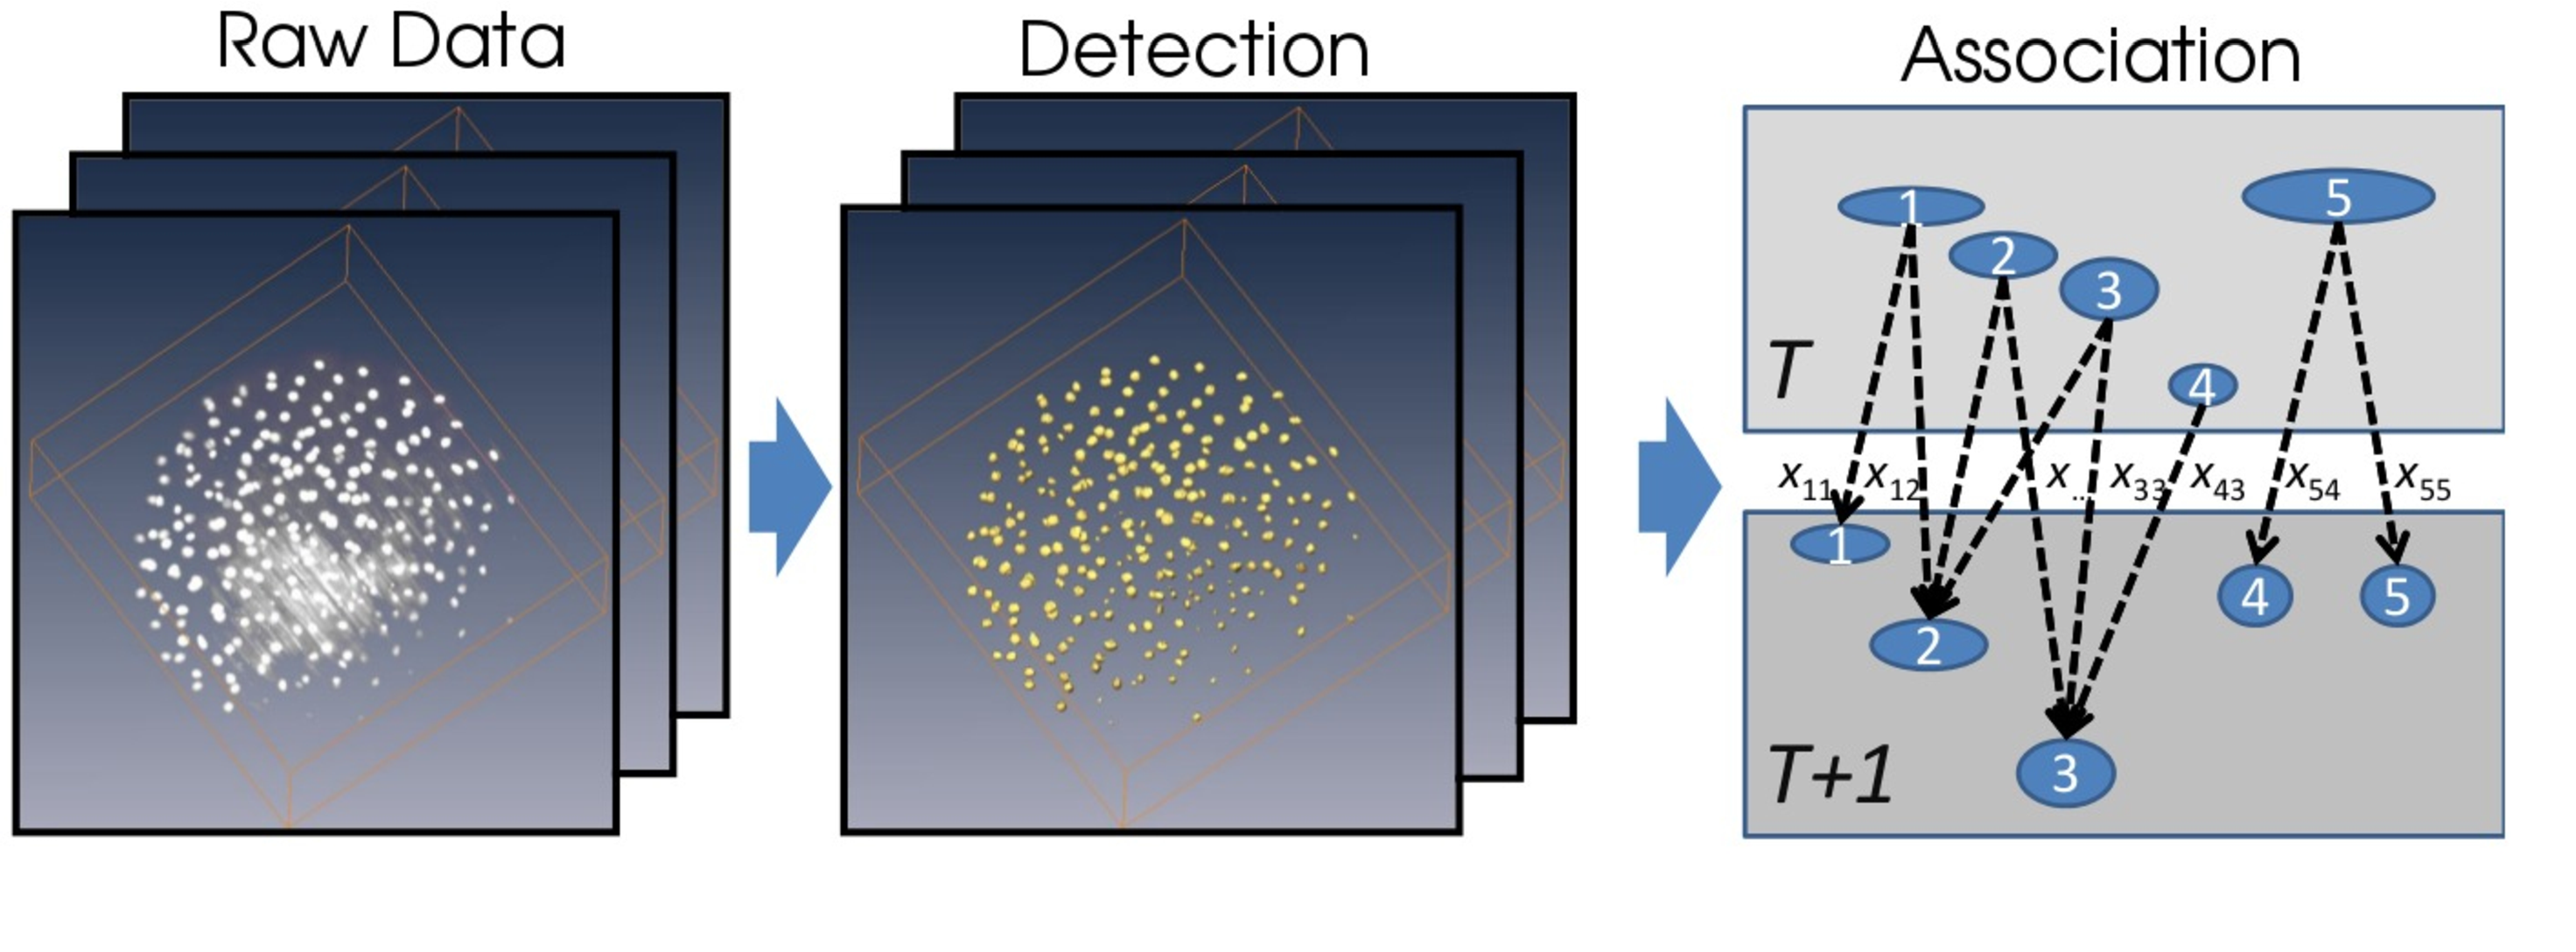
\includegraphics[width=\textwidth]{images/chaingraph/pipeline.pdf}
    %\rule{\textwidth}{0.3pt}
    \caption[Tracking-by-assignment pipeline]{Tracking-by-assignment pipeline, taken from
        \citet[9]{kausler_13_tracking}. Cell candidates are extracted from raw data by
        segmentation. Possible assignments (associations) are subsumed in the \emph{hypotheses
            graph}, as introduced by \citet[Chapter~3.1]{kausler_13_tracking}. The
        hypotheses graph does not describe a valid tracking (\eg cell $3$ in time step $T+1$ would
        have three parents), but a valid and optimal subset of the hypotheses can be concluded. Note
        that here assignment variables are described by $X_{ij}$. Throughout this thesis, variables
        named $X$ refer to detections, while assignments are referred to as $Y$.}
    \label{fig:cg-hypotheses}
\end{figure}


\subsection{Hypotheses Graph}
\newsavebox{\captionHypotheses}
\savebox{\captionHypotheses}{\small\tikz[baseline, inner
    sep=1pt]\node[thick, draw, circle, color=black, text=black] at (0,2.5pt){\tiny $X$};}

\label{subsec:hypotheses-graph}
The \emph{hypotheses graph} \citep[Chapter~3.1]{kausler_13_tracking} is a graphical
representation of possible assignments between cell detections. In general, any hypothetical
assignment between two cells is possible. However, in order to reduce the problem size, assignments
are restricted to cells in consecutive time steps. Moreover, only the $k$ nearest neighbors within a
thresholded distance at time step $t+1$ of a cell at time step $t$ are valid candidates for
assignment hypotheses, where $k$ is a design parameter of the model. In the graphical representation
of a toy example in \cref{fig:tba-hypotheses-graph} detections are depicted by nodes
({\protect\usebox{\captionHypotheses}}), while edges denote assignments. Note that, in general, the
position of the nodes in the hypotheses graph does not reflect the position of the corresponding
detections in raw data.

The tracking model is formulated as an algorithm that incorporates constraints and a quality measure
for feasible solutions in order to find the optimal tracking result. In the tracking models that are
discussed in this thesis (\cref{subsec:fg-chaingraph,subsec:fg-conservation,cha:joint}), these
constraints and measures are implemented in terms of a probabilistic graphical model.


\begin{figure}
    \centering
    \begin{subfigure}{0.44\textwidth}
        \centering
        \scalebox{0.9}{
            \begin{tikzpicture}[minimum size=58pt,scale=0.45, every node/.style={scale=0.45, text=black, font=\LARGE}, thick]
                    \begin{scope}
        \node (t1) {\huge $t$};
        \node[hypothesesdetection, below=of t1, circle, draw] (x11) {$X_1^t$};
        \node[hypothesesdetection, below=of x11, circle, draw] (x12) {$X_2^t$};
        \node[hypothesesdetection, below=of x12, circle, draw] (x13) {$X_3^t$};
    \end{scope}

    
    
    \begin{scope}
        \node[right=of t1, xshift=15mm] (t2) {\huge $t+1$};
        \node[hypothesesdetection, below=of t2, circle, draw] (x21) {$X_4^{t+1}$};
        \node[hypothesesdetection, below=of x21, circle, draw] (x22) {$X_5^{t+1}$};
    \end{scope}

    \begin{scope}[on background layer]
        \node[hypothesesdetection, below=of x22, circle, draw, on background layer] (x23) {$X_6^{t+1}$};
    \end{scope}
    
    
    \begin{scope}
        \node[right=of t2, xshift=15mm] (t3) {\huge $t+2$};
        \node[hypothesesdetection, below=of t3, circle, draw] (x31) {$X_7^{t+2}$};
        \node[hypothesesdetection, circle, draw, shift=($(x31.center)-(x21.center)$)] (x32) at (x22) {$X_8^{t+2}$};
    \end{scope}
    
    \begin{scope}[on background layer]
        \node[hypothesesdetection, below=of x32, circle, draw, on background layer] (x33) {$X_{10}^{t+2}$};
    \end{scope}
    
    % \begin{scope}
    %     \node[right=of t3, xshift=15mm] (t4) {\huge $t+3$};
    %     \node[hypothesesdetection, below=of t4, circle, draw] (x41) {$X_{10}^{t+3}$};
    %     \node[hypothesesdetection, below=of x41, circle, draw] (x42) {$X_{11}^{t+3}$};
    %     \node[hypothesesdetection, below=of x42, circle, draw] (x43) {$X_{12}^{t+3}$};
    % \end{scope}

    \begin{scope}[on background layer]
        \node[rectangle, draw, color=hypothesesbackground!40, fill=hypothesesbackground!30,
        fit=(x11) (x12) (x13), inner sep=13mm] (b1) {};
        \node[rectangle, draw, color=hypothesesbackground!40, fill=hypothesesbackground!30,
        fit=(x21) (x22) (x23), inner sep=13mm] (b2) {};
        \node[rectangle, draw, color=hypothesesbackground!40, fill=hypothesesbackground!30,
        fit=(b2), shift=($(t3.center) - (t2.center)$), inner sep=-0.1mm] (b3) {};
        % \node[rectangle, draw, color=hypothesesbackground!40, fill=hypothesesbackground!30,
        % fit=(x41) (x42) (x43), inner sep=13mm] (b4) {};
    \end{scope}

    \path[hypothesestransition] (x11) edge (x21);
    \path[hypothesestransition] (x12) edge (x22);
    \path[hypothesestransition] (x13) edge (x22);
    % \path[hypothesestransition] (x13) edge (x23);

    \path[hypothesestransition] (x21) edge (x31);
    \path[hypothesestransition] (x21) edge (x32);
    \path[hypothesestransition] (x22) edge (x32);
    % \path[hypothesestransition] (x23) edge (x32);

    % \path[hypothesestransition] (x31) edge (x41);
    % \path[hypothesestransition] (x32) edge (x42);
    % \path[hypothesestransition] (x32) edge (x43);

%%% Local Variables: 
%%% mode: latex
%%% TeX-master: "../../../main"
%%% End: 



%%% Local Variables: 
%%% mode: latex
%%% TeX-master: "../../main"
%%% End: 

            \end{tikzpicture}
        }
        \caption{Hypotheses Graph}
        \label{subfig:hypotheses-graph-example}
    \end{subfigure}
    \hfill
    \begin{subfigure}{0.44\textwidth}
        \centering
        \scalebox{0.9}{
            \begin{tikzpicture}[minimum size=58pt,scale=0.45, every node/.style={scale=0.45, text=black, font=\LARGE}, thick]
                    \begin{scope}
        \node (t1) {\huge $t$};
        \node[hypothesesdetection, below=of t1, circle, draw] (x11) {$X_1^t$};
    \end{scope}
    \begin{scope}[on background layer]
        \node[hypothesesdetection, below=of x11, circle, draw] (x12) {$X_2^t$};
    \end{scope}
    \begin{scope}
        \node[hypothesesdetection, below=of x12, circle, draw] (x13) {$X_3^t$};
    \end{scope}

    
    
    \begin{scope}
        \node[right=of t1, xshift=15mm] (t2) {\huge $t+1$};
        \node[hypothesesdetection, below=of t2, circle, draw] (x21) {$X_4^{t+1}$};
        \node[hypothesesdetection, below=of x21, circle, draw] (x22) {$X_5^{t+1}$};
    \end{scope}

    \begin{scope}[on background layer]
        \node[hypothesesdetection, below=of x22, circle, draw, on background layer] (x23) {$X_6^{t+1}$};
    \end{scope}
    
    
    \begin{scope}
        \node[right=of t2, xshift=15mm] (t3) {\huge $t+2$};
        \node[hypothesesdetection, below=of t3, circle, draw] (x31) {$X_7^{t+2}$};
        \node[hypothesesdetection, circle, draw, shift=($(x31.center)-(x21.center)$)] (x32) at (x22) {$X_8^{t+2}$};
    \end{scope}
    
    \begin{scope}[on background layer]
        \node[hypothesesdetection, below=of x32, circle, draw, on background layer] (x33) {$X_{10}^{t+2}$};
    \end{scope}
    
    % \begin{scope}
    %     \node[right=of t3, xshift=15mm] (t4) {\huge $t+3$};
    %     \node[hypothesesdetection, below=of t4, circle, draw] (x41) {$X_{10}^{t+3}$};
    %     \node[hypothesesdetection, below=of x41, circle, draw] (x42) {$X_{11}^{t+3}$};
    %     \node[hypothesesdetection, below=of x42, circle, draw] (x43) {$X_{12}^{t+3}$};
    % \end{scope}

    \begin{scope}[on background layer]
        \node[rectangle, draw, color=hypothesesbackground!40, fill=hypothesesbackground!30,
        fit=(x11) (x12) (x13), inner sep=13mm] (b1) {};
        \node[rectangle, draw, color=hypothesesbackground!40, fill=hypothesesbackground!30,
        fit=(x21) (x22) (x23), inner sep=13mm] (b2) {};
        \node[rectangle, draw, color=hypothesesbackground!40, fill=hypothesesbackground!30,
        fit=(b2), shift=($(t3.center) - (t2.center)$), inner sep=-0.1mm] (b3) {};
        % \node[rectangle, draw, color=hypothesesbackground!40, fill=hypothesesbackground!30,
        % fit=(x41) (x42) (x43), inner sep=13mm] (b4) {};
    \end{scope}

    \path[hypothesestransition] (x11) edge (x21);
    % \path[hypothesestransition] (x12) edge (x22);
    \path[hypothesestransition] (x13) edge (x22);
    % \path[hypothesestransition] (x13) edge (x23);

    \path[hypothesestransition] (x21) edge (x31);
    % \path[hypothesestransition] (x21) edge (x32);
    \path[hypothesestransition] (x22) edge (x32);
    % \path[hypothesestransition] (x23) edge (x32);

    % \path[hypothesestransition] (x31) edge (x41);
    % \path[hypothesestransition] (x32) edge (x42);
    % \path[hypothesestransition] (x32) edge (x43);

%%% Local Variables: 
%%% mode: latex
%%% TeX-master: "../../../main"
%%% End: 



%%% Local Variables: 
%%% mode: latex
%%% TeX-master: "../../main"
%%% End: 

            \end{tikzpicture}
        }
        \caption{Possible tracking result}
        \label{subfig:hypotheses-graph-example-inferred}
    \end{subfigure}
    \caption[Exemplary hypotheses graph]{Exemplary hypotheses graph
        (\subref{subfig:hypotheses-graph-example}) with a potential, meaningful tracking result
        (\subref{subfig:hypotheses-graph-example-inferred}). Detections are represented by black
        circles, edges show assignment hypotheses. False positive detections and hypotheses are
        removed from the hypotheses graph after inference. The tracker decided, that $X_2^t$ was a
        false detection and corrected that error.}
    \label{fig:tba-hypotheses-graph}
\end{figure}

% $\protect\usebox{\captionTest}$,

%%% Local Variables: 
%%% mode: latex
%%% TeX-master: "../../main"
%%% End: 

\section{Tracking as a Factor Graph}
\label{sec:tracking-as-a-factor-graph}
The tracking-by-assignment problem can be solved using probabilistic graphical models. For that
purpose, random variables for the assignments and detections are introduced, thus imposing
uncertainty. These random variables are used to construct a graphical model from the tracking
hypotheses whose specific form is a design choice of the tracking approach. The optimal solution is
then deduced by performing inference on the graphical model. In general, it is reasonable to
transfer the graphical model into a factor graph before inference, if not already formulated as a
factor graph directly.

In the following, two approaches are described, that utilize the power of probabilistic graphical
models, namely \emph{chain graph} tracking in \cref{subsec:fg-chaingraph} and \emph{conservation}
tracking in \cref{subsec:fg-conservation}. While the chain graph approach uses a \emph{chain graph},
\ie a graphical model with both directed and undirected edges
(\citealp[Chapter~4.1.5]{kausler_13_tracking};
\citealp[Chapter~4.6.2]{koller_09_probabilistic},
\citealp{frydenberg_90_chain}), for modeling and a factor graph for inference, the
conservation tracking models a factor graph directly.

\subsection{Chain Graph Tracking}
\label{subsec:fg-chaingraph}
\citet{kausler_12_discrete} introduce a graphical model approach for tracking-by-assignment. Based
on a cell \vs background segmentation, they first generate tracking hypotheses -- \ie possibly
ambiguous assignments of objects at time $t$ to objects at time $t+1$ -- that are subsumed in the
hypotheses graph. Nodes in the hypotheses graph represent detections. Edges between these nodes
correspond to assignment hypotheses. Furthermore, a node is called active, if inference determined
the corresponding detection to be a true positive detection. Similarly, an active edge means that a
potential assignment turned out to be true after inference. After inference, a subset of these edges
and nodes represents a biologically meaningful tracking, if it fulfills the following constraints:
\begin{enumerate}
      \item A node cannot have more than two active outgoing edges, \ie a cell cannot divide into
    more than two children cells.
      \item A node cannot have more than one active incoming edge, \ie a cell must have a single or
    no ancestor.
      \item An edge cannot be active if at least one of the nodes it is connected to is
    a false positive (inactive), \ie an assignment from/to a cell to/from background is not possible.
\end{enumerate}
Then, the tracking task can be reinterpreted as a labeling problem on the hypotheses graph that is
solved using graphical models.  For that purpose, \citet{kausler_12_discrete} introduce two kinds of
binary random variables:
\begin{enumerate}
      \item Assignment variables $Y_{ij}^{(t)}, \val\left(Y_{ij}^{(t)}\right)=\{0,1\}$ indicate whether an
    assignment from cell $i$ at time $t$ to cell $j$ at time $t+1$ is active ($1$) or inactive
    ($0$). The set of all assignment variables at time $t$ is denoted by $\mathcal{Y}^{(t)}$. For
    completeness, $\mathcal{Y}$ is the set of all assignment variables in the model.
      \item Detection variables $X_i^{(t)}, \val\left(X_i^{(t)}\right)=\{0,1\}$ indicate whether a detection
    is a false positive (inactive, $0$) or a true detection (active, $1$). Analogously to the
    notation for assignment variables, $\mathcal{X}^{(t)}$ denotes the set of all detection
    variables at time $t$ and $\mathcal{X}$ stands for all detection variables in the model.
\end{enumerate}

These random variables are brought into relation in a \emph{chain graph} representation of the
hypotheses graph, \ie a graphical model that contains both directed and undirected edges. In
addition, there may be no directed cycles in a chain graph. Generally, chain graphs are beyond the
scope of this thesis and further details are given in \citet[][Chapter~4.1.5]{kausler_13_tracking},
\citet[][Chapter~4.6.2]{koller_09_probabilistic}, \citet{frydenberg_90_chain}.

The undirected part of this chain graph model is formed by ``supernodes'' for all pairs of
consecutive time steps $t$, $t+1$. Each of these supernodes consists of a a conditional random field
(\cref{subsec:gm-crf}) describing the joint probability
\begin{align}
    \label{eq:chaingraph-crf}
    P^{(t)}(\mathcal{Y}^{(t)}|\mathcal{X}^{(t)},\mathcal{X}^{(t+1)})= \frac{1}{Z^{(t)}} %(\mathcal{X}^{(t)},\mathcal{X}^{(t+1)})}
    \!\!\!\!\prod_{X_i^{(t)}\in\mathcal{X}^{(t)}}\!\!\!\!\!\!\!\phi^{(t)}_{i\rightarrow}(X_i^{(t)},\mathcal{Y}^{(t)}_{i\rightarrow})\!\!\!\!\!\!\!\! \prod_{X_j^{(t+1)}\in\mathcal{X}^{(t+1)}}\!\!\!\!\!\!\!\!\!\!\!\!\phi^{(t)}_{\rightarrow
        j}(\mathcal{Y}^{(t)}_{\rightarrow j},X_j^{(t+1)}),
\end{align}
over all assignment variables $\mathcal{Y}^{(t)}$ between time steps $t$ and $t+1$ conditioned on the
corresponding detection variables $\mathcal{X}^{(t)}$ and $\mathcal{X}^{(t+1)}$ (see also
\cref{fig:chaingraph-crf}). These supernodes in conjunction with the detection variables form a
directed graphical model (Bayesian network, \cref{subsec:gm-bayesian-net}) as depicted in
\cref{fig:chaingraph-bn}. With the prior probability $P_{\text{det}}(X_i^{(t)})$ that a detection is
a true detection, the joint probability for $\mathcal{X}$ and $\mathcal{Y}$ over all time steps
factorizes as
\begin{align}
\label{eq:chaingraph-prob}
P(\mathcal{X},\mathcal{Y})= 
\prod_{t=1}^T\prod_{X_i^{(t)}\in\mathcal{X}^{(t)}}\!\!\!\!\!\! P_{\mathrm{det}}(X_i^{(t)})\cdot\prod_{t=1}^{T-1}P^{(t)}(\mathcal{Y}^{(t)}|\mathcal{X}^{(t)},\mathcal{X}^{(t+1)}).
\end{align}
This probability distribution can be expressed as a Gibbs distribution of a factor graph
\begin{align}
    \label{eq:cg-gibbs}
    P(\mathcal{X},\mathcal{Y})&=\frac{1}{Z}e^{-\log E(\mathcal{X},\mathcal{Y})} \\
     E(\mathcal{X},\mathcal{Y}) &= 
     \!\sum_{t=1}^{T} \!\!\!\!\! \sum_{\ \ X_i^{(t)}\in
         \mathcal{X}^{(t)}}\!\!\!\!\!\!\!\!\!  E_{\mathrm{det}}(X_i^{(t)})+
     \sum_{t=1}^{T-1} \!\! \left( \!\! \sum_{i}E_{\mathrm{out}}(X_i^{(t)},\mathcal{Y}_{i\rightarrow}^{(t)})+ \!\!
         \sum_{j} \! E_{\mathrm{in}}(\mathcal{Y}_{\rightarrow
             j}^{(t)},X_j^{(t+1)})\!\! \right) 
    % E(\mathcal{X},\mathcal{Y})&=\sum_{t+1}^T\sum_{X_i^{(t)}\in\mathcal{X}^{(t)}E_{det}(X_i^{(t)})+
    % \sum_{t=1}^{T-1}\left(\sum_iE_{out}\left(X_i^{(t)},\mathcal{Y_
\end{align}
over detection variables $\mathcal{X}$ and assignment variables $\mathcal{Y}$. The energies in
\cref{eq:cg-gibbs} correspond to factors in the factor graph representation of the chain graph
model. They assign giving low energies to configurations that represent a meaningful tracking and
disallow configurations that would not result in a sensible tracking. In terms of probabilities, a
low energy means a high probability and vice versa. More accurately, they are defined as the
outgoing energy


\begin{subnumcases}{\label{eq:cg-cost-out} E_{\mathrm{out}}(X_i^{(t)},\mathcal{Y}_{i\rightarrow}^{(t)}) = }
    \infty,&$X_i^{(t)}=1\wedge\sum_j Y_{i
        j}^{(t)}>2 \quad$  \label{eq:cg-cost-out-a}\\
    E_{\text{div}}(X_i^{(t)},\mathcal{Y}_{i\rightarrow}^{(t)}),&$X_i^{(t)}=1\wedge\sum_j
    Y_{ij}^{(t)}=2$  \label{eq:cg-cost-out-b}\\
    E_{\text{move}}(X_i^{(t)},\mathcal{Y}_{i\rightarrow}^{(t)}),&$X_i^{(t)}=1\wedge\sum_j Y_{i
        j}^{(t)}=1$  \label{eq:cg-cost-out-c}\\
    C_{\text{dis}},&$X_i^{(t)}=1\wedge\sum_j
    Y_{ij}^{(t)}=0$  \label{eq:cg-cost-out-d}\\
    C_{\text{opp}},&$X_i^{(t)}=0\wedge\sum_j
    Y_{ij}^{(t)}=0$  \label{eq:cg-cost-out-e}\\
    \infty,&$X_i^{(t)}=0\wedge\sum_j Y_{i
        j}^{(t)}>0$ \label{eq:cg-cost-out-f}
\end{subnumcases}

\begin{align}
    \label{eq:cg-cost-energies}
     E_{\text{div}}(X_i^{(t)},\mathcal{Y}_{i\rightarrow}^{(t)}) &= w\sum_j Y_{ij}^{(t)}\cdot
     (d_j-\bar{d})^2, \\
     E_{\text{move}}(X_i^{(t)},\mathcal{Y}_{i\rightarrow}^{(t)}) &= w\sum_j Y_{ij}^{(t)}\cdot
     d_j^2,
\end{align}

with $d_j$ denoting the distance of the two cells joined by assignment $Y_{ij}$ and $\bar{d}$
standing for the average distance of a child cell from the dividing parent cell. The outgoing energy
$E_{\mathrm{out}}(X_i^{(t)},\mathcal{Y}_{i\rightarrow}^{(t)})$
\begin{itemize}
      \item disallows illegal configurations, \ie a division into more than two children
    (\ref{eq:cg-cost-out-a}) and a transition where a detection has been marked false positive (\ref{eq:cg-cost-out-f}), by
    assigning $\infty$,
      \item assigns the squared deviations of the parent-children distances to the average
    parent-child distance, weighted by design parameter $w$, in case of a
    division (\ref{eq:cg-cost-out-c}),
      \item assigns the squared distance between a cell and its predecessor  (\ref{eq:cg-cost-out-b}),
      \item assigns the constant disappearance cost $C_{\text{dis}}$, if the cell vanishes  (\ref{eq:cg-cost-out-d}), and finally
      \item assigns the constant opportunity cost $C_{\text{opp}}$ if nothing happens
    (\ref{eq:cg-cost-out-e}), \ie in case of a false positive detection, in order to bias the result
    towards activating cells rather then deactivating them.
\end{itemize}

Secondly, the incoming energy

% \begin{align}
% \resizebox{0.9\hsize}{!}{$
% E_{\mathrm{out}}(X_i^{(t)},\mathcal{Y}_{i\rightarrow}^{(t)}) = \left\{
% \begin{array}{ll|l}
%         \infty&\!\!\!,X_i^{(t)}=1\wedge\sum_j Y_{i
% j}^{(t)}>2 \quad & \ > 2\text{ children}\\
%         \begin{array}{l}\!w\bigl((d-\bar{d})^2
% \\\!+(d'-\bar{d})^2\bigr)\end{array}&\!\!\!,X_i^{(t)}=1\wedge\sum_j
% Y_{ij}^{(t)}=2 & \ \text{division}\\
%         wd^2&\!\!\!\!,X_i^{(t)}=1\wedge\sum_j Y_{i
% j}^{(t)}=1 & \ \text{move}\\
%         C_{\mathrm{term}}&\!\!\!\!,X_i^{(t)}=1\wedge\sum_j
% Y_{ij}^{(t)}=0 & \ \text{disappearance}\\
%         C_{\mathrm{opp}}&\!\!\!\!,X_i^{(t)}=0\wedge\sum_j
% Y_{ij}^{(t)}=0 & \ \text{opportunity}\\
%         \infty&\!\!\!\!,X_i^{(t)}=0\wedge\sum_j Y_{i
% j}^{(t)}>0 & \ \text{tracked misdetection}
%     \end{array}\right.
% $}
% \end{align}

\begin{subnumcases}{\label{eq:cg-cost-in} E_{\mathrm{in}}(\mathcal{Y}_{\rightarrow j}^{(t)},X_j^{(t+1)}) =}
    \infty,&$X_j^{(t+1)}=1\wedge\sum_i Y_{i
        j}^{(t)}>1$ \label{eq:cg-cost-in-a}\\
    0,&$X_j^{(t+1)}=1\wedge\sum_i Y_{i
        j}^{(t)}=1$\label{eq:cg-cost-in-b}\\
    C_{\mathrm{app}},&$X_j^{(t+1)}=1\wedge\sum_i Y_{i
        j}^{(t)}=0$\label{eq:cg-cost-in-c}\\
    0,&$X_j^{(t+1)}=0\wedge\sum_i Y_{i
        j}^{(t)}=0$\label{eq:cg-cost-in-d}\\
    \infty,&$X_j^{(t+1)}=0\wedge\sum_i Y_{i
        j}^{(t)}>0$\label{eq:cg-cost-in-e}
\end{subnumcases}
assigns
\begin{itemize}
      \item zero energy to move (\ref{eq:cg-cost-in-b}) and empty (\ref{eq:cg-cost-in-d}), false
    positive detection and no transition) configurations (already covered by $E_{\text{out}}$),
      \item infinity to illegal configurations \ie a cell with more than one predecessor (\ref{eq:cg-cost-in-a}) or an
    active transition when the detection is labeled false positive (\ref{eq:cg-cost-in-e}), and finally
      \item constant appearance cost $C_{\text{app}}$ in case of an appearing cell with no
    predecessor (\ref{eq:cg-cost-in-c}).
\end{itemize}

Finally, the detection energy
\begin{align}
    \label{eq:chaingraph-cost-det}
    E_{\mathrm{det}}\left(X_i^{(t)}\right)=
    \begin{cases}
        -\ln\left(\hat{P}_{\mathrm{det}}\left(X_i^{(t)}\right)\right)&,X_i^{(t)}=1\\
        -\ln\left(1-\hat{P}_{\mathrm{det}}\left(X_i^{(t)}\right)\right)&,X_i^{(t)}=0
    \end{cases}
\end{align}
is determined by the prediction $\hat{P}_{\mathrm{det}}$ of a trained random forest cell
classifier~(\cref{cha:app-rf}) which gives an estimate on how likely it is that a detection is an
actual cell.

For the computation of the MAP solution which reflects the optimal configuration, the authors choose
to use an ILP for inference as shown in \cref{subsec:factor-graphs} which produces a globally optimal
solution and, furthermore, gives the advantage of excluding illegal configurations with infinite
energies by means of hard constraints.



\begin{figure}[h]
    \centering
    \begin{subfigure}[t]{0.48\textwidth}
        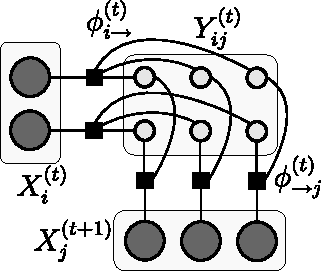
\includegraphics[width=\textwidth]{images/chaingraph/fig_crf_less_nodes.pdf}
        %\rule{\textwidth}{0.3pt}
        \caption{Factor graph representation of the conditional random field at time steps $t$ and
            $t+1$, \ie the undirected part of the chain graph. The assignment variables (smaller,
            light nodes) $Y_{ij}^{(t)}$ are conditioned on the detection variables
            $X_i^{(t)},X_i^{(t+1)}$(dark nodes).}
        \label{fig:chaingraph-crf}
    \end{subfigure}
    \hfill
    \begin{subfigure}[t]{0.48\textwidth}
        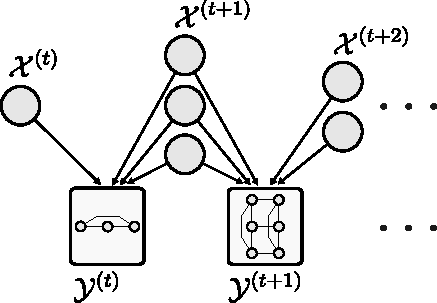
\includegraphics[width=\textwidth]{images/chaingraph/fig_chain_graph.pdf}
        %\rule{\textwidth}{0.3pt}
        \caption{In the directed part of the chain graph the conditional random fields from
            \cref{fig:chaingraph-crf} are subsumed in supernodes (boxes).}
        \label{fig:chaingraph-bn}
    \end{subfigure}
    \caption[Chain graph model]{Conditional random field representation for two consecutive time steps
        of the ``transition model'' (\subref{fig:chaingraph-crf}) and chain graph model for three
        subsequent time steps (\subref{fig:chaingraph-bn}), taken from \citet{kausler_12_discrete}.}
    \label{fig:chaingraph-model}
\end{figure}

After the recap of the chain graph tracking and the conservation tracking factor graph in
\cref{subsec:fg-chaingraph,subsec:fg-conservation}, respectively, we continue with the introduction
of cell identity reconstruction for conservation tracking~(\cref{cha:GMM}) and a new
tracking-by-assignment method, joint segmentation and tracking~(\cref{cha:joint}), which both
address the problem of undersegmentation in cell tracking.


%%% Local Variables: 
%%% mode: latex
%%% TeX-master: "../../../main"
%%% End: 



\subsection{Conservation Tracking}
\label{subsec:fg-conservation}

The chain graph tracking as described above is capable of handling an unknown number of dividing
objects, if each detection contains one cell at maximum. This means that the segmentation must
contain all cells in the data set as individual objects in order to achieve an accurate tracking
result. As a consequence, speckle noise (false positives) can be handled by chain graph tracking.
``Mergers'' however, that may occur by occlusions in 2d or due to bad imaging quality in 2d and 3d,
pose an obstacle for the chain graph tracking: When two or more cells are merged into a single
connected component due to undersegmentation, all but one of the associated tracks will get lost, as
the chain graph energies (Equations~\ref{eq:cg-cost-out} to~\ref{eq:chaingraph-cost-det}) disallow merging, \ie a
cell has more than once ancestor. From a chain graph tracking point of view, the lost tracks appear
either as disappearances or a series of false positive detections in the time steps previous to the
merging event. In a similar fashion, a demerging of a merger object cannot be handled correctly by
the chain graph tracking either. Here, the chain graph tracking would interpret the incident as a
transition from the merged object to one of its possible descendants in the next time step in
conjunction with either one or more appearances or false positive detections. Furthermore, a
demerging of two cells might be misinterpreted as a division.

Since unique detections of all cells cannot be guaranteed in dense cell populations or poor image
quality, \citet{schiegg_13_conservation} propose a method that can also handle merges. They leave
behind the assumption that a detection matches exactly one cell or is a false positive. In terms of
graphical models, this means that, in contrast to the chain graph tracking model, the random
variables are not binary, but discrete variables that carry information about how many cells they
represent (one detection variable still represents a single detection). They then apply conservation
laws that ensure ``global consistency of the solution''. This allows for detection of merged cells,
\ie detections that represent more than one cell. A more detailed description of this method is
provided in the following including an overview of the pipeline in
\cref{fig:fg-conservation-pipeline}. Reconstruction of the identities of the involved cells requires
an additional post-processing step which is our contribution and will be discussed in detail in
\cref{cha:GMM}.

\begin{figure}
    \centering
    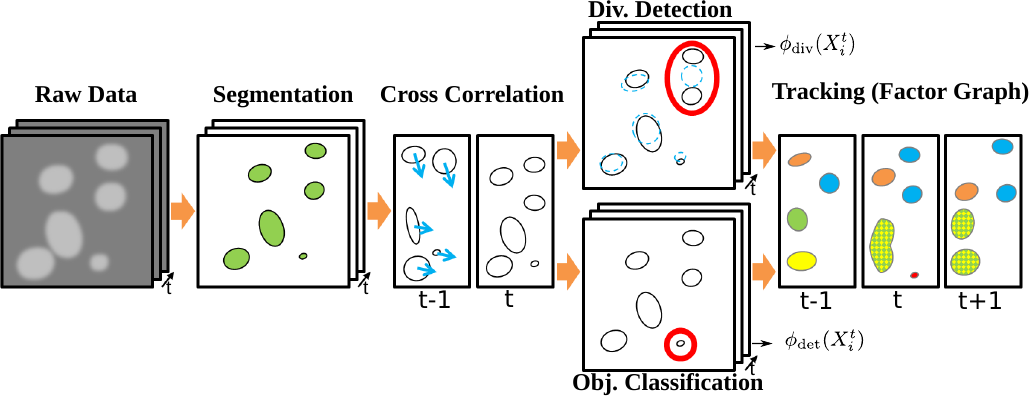
\includegraphics[width=\textwidth]{images/conservation/pipeline.png}
    %\rule{\textwidth}{0.3pt}
    \caption[Conservation tracking pipeline]{Pipeline of the conservation tracking (taken and modified
        from~\cite{schiegg_13_conservation}): First cells are detected in the segmentation
        step. Then, cross correlation is used for estimating the cell positions in subsequent
        time steps. Based on these corrected positions, the hypotheses graph is generated. Finally,
        inference on the corresponding factor graph yields a tracking result. In order to inject
        prior belief, the predictions of classifiers for divisions and the number of objects in a
        detection are taken into account in the potentials of the factor graph.} 
    \label{fig:fg-conservation-pipeline}
\end{figure}

\citet{schiegg_13_conservation} use a factor graph for modeling. To this end, they introduce
discrete multi-state random variables for detections, $X_i^t \in \{0,\dots ,m\}$,
representing connected component $i$ at time step $t$. The state of such a detection variable
determines the number of cells that are comprised in the corresponding connected
component. Additionally, transition random variables $T_{ij}^t, \in \val(T_{ij}^t)=\{0,\dots ,m\}$
represent transitions from detection $i$ at time $t$ to detection $j$ at time $t+1$. Here, the
design parameter $m$ specifies the maximum allowed number of cells per connected
component. Moreover, the transition variables can be interpreted as some ``flow'' of mass going from
detection $i$ at time $t$ to detection $j$ at time $t+1$. Then, conservation laws, hence the name
``conservation tracking'', ensure global consistency. However, appearances and disappearances are
not consistent with these conservation laws. Therefore, to allow for breaking these laws, $X_i^t$
is defined deterministically as
\begin{align}
    \label{eq:cons-det-a-v}
    X_i^t& = \max(V_i^t, A_i^t), \\
    \val(V_i^t) &= \val(A_i^t) = \{0,\dots ,m\},
\end{align}
with discrete random variables $V_i^t$ and $A_i^t$, which need not follow conservation laws, thus
making appearances and disappearances possible. Then an appearance is modeled by $V_i^t=0,
A_i^t=k>0$ (Equation~\ref{eq:fg-conservation-det-b} and a disappearance by $V_i^t=k>0, A_i^t=0$
(Equation~\ref{eq:fg-conservation-det-c}). Therefore, partial appearances or disappearances are not
possible (Equation~\ref{eq:fg-conservation-det-d}). On the contrary, $V_i^t=A_i^t$
(Equation~\ref{eq:fg-conservation-det-c}) represents a connected component, which does not appear or
disappear, \ie it has possibly multiple ancestors and descendants, with the special case of a false
positive detection $V_i^t=A_i^t=0$.
% representing the event of disapperance and
% appearance respectively. This is neccessary because an appearance means, that no mass is flowing
% into the cell, which would be a violation of the conservation law. This holds for disappearances
% analogously. Thus, the conservation law between vanishing and appearing nodes needs to be redefined:
% Both variables may be in the same state, representing a false positive detection in case of state
% zero and a transition otherwise. Moreover, either of the variables may be zero while the other is
% non-zero. This is the case when a cell disappears or appears. A partial appearance or disappearance
% is not allowed, which is enforced by disallowing configurations where vanishing and appearaing
% variable are both non-zero, but not in the same state.

Furthermore, to distinguish between a division and the demerging into two single cells, a
binary division variable $D_i^t \in \{0, 1\}$ is introduced that indicates whether a cell is dividing
into two children cells, or not.

\cref{fig:conservation-fg} shows how these random variables are brought into relation in a factor
graph. In order to pull the configuration of random variables towards a meaningful tracking
solution, the factors of this graph score configurations by assigning a high energy to states that
are unlikely to resemble a real tracking while keeping the energy of more likely, preferable
configurations low. Moreover, they disallow illegal configurations as specified above.

\begin{figure}
    \centering
    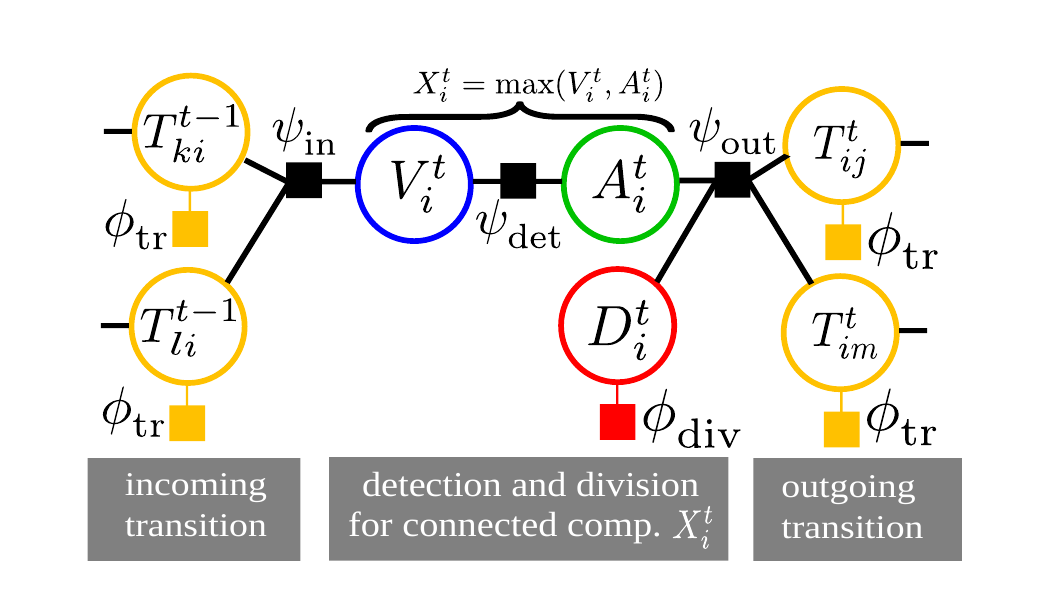
\includegraphics[width=0.6\textwidth]{images/conservation/factor_graph.png}
    %\rule{\textwidth}{0.3pt}
    \caption[Conservation tracking factor graph]{Factor graph of the conservation tracking model
        (taken from \citet{schiegg_13_conservation}): The excerpt of the factor graph shows
        variables that share potentials with a transition node, or, more precisely, with the
        vanishing node and the appearing node, that determine the state of the transition node.}
    \label{fig:conservation-fg}
\end{figure}

In the following, the factors are specified. To begin with, the \emph{detection factor}
\begin{align}
    \label{eq:fg-conservation-det}
    \psi_{\text{det}}(A_i^t,V_i^t,f_i^t) &= e^{-E_{\text{det}}(A_i^t,V_i^t,f_i^t)},
\end{align}
\begin{subnumcases}{E_{\text{det}}(A_i^t,V_i^t,f_i^t) =}
    -\log\bigl(\hat{P}(X_i^t=k|f_i^t)\bigr), &$V_i^t=A_i^t=k$ \label{eq:fg-conservation-det-a}\\
    -\log\bigl(\hat{P}(X_i^t=k|f_i^t)\bigr) + kw_{\text{app}}, &$V_i^t=0, A_i^t=k > 0$ \label{eq:fg-conservation-det-b}\\
    -\log\bigl(\hat{P}(X_i^t=k|f_i^t)\bigr) + kw_{\text{dis}}, &$V_i^t=k > 0, A_i^t=0$ \label{eq:fg-conservation-det-c}\\
    \infty, &$\text{otherwise}$ \label{eq:fg-conservation-det-d}
\end{subnumcases}
takes into account local evidence $f_i^t$, \eg size or mean, and weighs configurations according to
their probability $\hat{P}(X_i^t=k|f_i^t)$ that a connected component contains
\mbox{$k\in\{0,\hdots,m\}$} cells given $f_i^t$, as determined by a random forest
classifier~(Equations~\ref{eq:fg-conservation-det-a} to \ref{eq:fg-conservation-det-c}, \cref{cha:app-rf}). The design
parameter $m$ specifies the maximum number of cells per connected component, whereas the design
parameters $w_{\text{app}}$ and $w_{\text{dis}}$ are penalties for appearing and disappearing cells
respectively. Furthermore, $E_{\text{det}}$ forbids illegal configurations by assigning infinite
energy (Equation \ref{eq:fg-conservation-det-d}), corresponding to zero probability.

Secondly, unary factors on the transitions
\begin{align}
    \label{eq:fg-conservation-trans}
    -\log\left(\phi_{\text{tr}}(T_{ij}^t,d_{ij}^t)\right) = E_{\text{tr}}(T_{ij}^t,d_{ij}^t) = -w_{\text{tr}}
    \begin{cases}
        1-\exp\left(-\frac{d_{ij}^t}{\alpha}\right), & T_{ij}^t=0 \\
        \exp\left(-\frac{d_{ij}^t}{\alpha}\right), & T_{ij}^t > 0
    \end{cases}
\end{align}
are constructed by the squared difference between the two cells involved in the potential transition
with design parameters $\alpha$ and $w_{\text{tr}}$. As an additional feature, the authors estimate the position of a
cell in the subsequent time step and calculate the squared distance with respect to that
position. This is a penalty on the acceleration rather than on the velocity of a cell, which
represents natural behavior in a better way. More precisely, the position estimate is the result of
performing patch-wise cross correlation~\citep[Chapter~14.5]{jaehne_05_digital} on successive frames of the binary segmentation.

In a similar fashion, unary factors on the division variables
\begin{align}
    \label{eq:fg-conservation-div}
    -\log\left(\phi_{\text{div}}(D_i^t, f_i^t)\right) = &E_{\text{div}}(D_i^t, f_i^t) \\= &-w_{\text{div}}
    \begin{cases}
        \log\left(1-\hat{P}(D_i^t=1|f_i^t)\right), & D_i^t = 0 \\
        \log\left(\hat{P}(D_i^t=1|f_i^t\right), & D_i^t = 1
    \end{cases}
\end{align}
embody the probability that a cell is about to divide, provided by a random forest 
classifier trained on cell detections. Again, $f_i^t$ describes local features and $w_{\text{div}}$
is a design parameter that -- like $w_{\text{tr}}$ -- weights the division prior against the
detection prior.

Finally, the conservation laws are implemented as constraints in the outgoing factor
\begin{align}
    \label{eq:fg-conservation-out}
    \psi_{\text{out}}(A_i^t, T_{ij_1}^t,\dots ,T_{ij_n}^t) = e^{-E_{\text{out}}(A_i^t, T_{ij_1}^t,\dots ,T_{ij_n}^t)},
\end{align}
\begin{subnumcases}{\label{eq:cons-out} E_{\text{out}}(A_i^t, T_{ij_1}^t,\dots ,T_{ij_n}^t) =}
    \infty, & $\sum_{l\in \{j_1,\dots , j_n\}} T_{il}^t \ne A_i^t + D_i^t$ \label{eq:cons-out-a} \\
    \infty, & $\exists l \in \{j_1,\dots , j_n\}: T_{il}^t > A_i^t$ \label{eq:cons-out-b}\\
    \infty, & $\sum_{l\in \{j_1,\dots , j_n\}} T_{il}^t \ne 2 \text{ if } D_i^t =
    1$ \label{eq:cons-out-c} \\
    \infty, & $A_i^t \ne 1 \text{ if } D_i^t = 1$ \label{eq:cons-out-d} \\
    0, & $\text{otherwise}$ \label{eq:cons-out-e}
\end{subnumcases}
and in the incoming factor analogously. These constraints have a meaningful interpretation in the
context of mass conservation laws: Equation \ref{eq:cons-out-a} ensures conservation of mass from a
detection to the corresponding outgoing transitions. In case of a division, the additional mass is
created by the division variable (Equations \ref{eq:cons-out-a} and
\ref{eq:cons-out-b}). Furthermore, a merger cannot be a dividing object (Equation
\ref{eq:cons-out-d}). In conjunction with Equations \ref{eq:cons-out-a} and \ref{eq:cons-out-c},
this implies that a division cell must have exactly two children and that the mass involved in a
division is $2$, equally distributed on the division variable and the detection variable.

The product of all of these factors, divided by the partition function $Z$ defines the probability for
a specific configuration of all random variables:
\begin{align}
    \label{eq:fg-conservation-prob}
    P(\mathcal{A}, \mathcal{V}, \mathcal{D}, \mathcal{T}) = \frac{1}{Z}\prod_t\prod_i \Biggl(
    &\psi_{\text{det}}\left(A_i^t,V_i^t,f_i^t\right ) \phi_{\text{div}}\left(D_i^t\right)
    \prod_j\left(\phi_{\text{tr}}(T_{ij}^t)\right) \\\nonumber \times &\psi_{\text{out}}\left(A_i^t,
        T_{ij_1}^t,\hdots T_{ij_n}^t\right) \psi_{\text{in}}\left(A_i^t, T_{h_1i}^{t-1},\hdots
        T_{h_ni}^{t-1}\right) \Biggr)
\end{align}

Just as in the chain graph tracking (\cref{subsec:fg-chaingraph}), the MAP solution is inferred by
reformulating \cref{eq:fg-conservation-prob} as a Gibbs energy that is minimized in an ILP:
\begin{align}
    \argmax_{\mathcal{A}, \mathcal{V}, \mathcal{D}, \mathcal{T}}P(\mathcal{A}, \mathcal{V},
    \mathcal{D}, \mathcal{T}) & = \argmin_{\mathcal{A}, \mathcal{V}, \mathcal{D}, \mathcal{T}} E(\mathcal{A}, \mathcal{V}, \mathcal{D}, \mathcal{T}) \\
    &= \argmin_{\mathcal{A}, \mathcal{V}, \mathcal{D}, \mathcal{T}}\left(-\log P(\mathcal{A},
        \mathcal{V}, \mathcal{D}, \mathcal{T})\right).
    \label{eq:fg-conservation-map}
\end{align}

%%% Local Variables: 
%%% mode: latex
%%% TeX-master: "../../../main"
%%% End: 

%%% Local Variables: 
%%% mode: latex
%%% TeX-master: "../../main"
%%% End: 


%%% Local Variables: 
%%% mode: latex
%%% TeX-master: "../main"
%%% End: 
